%%%%%%%%%%%%%%%%%%%%%%%%%%%%%%%%%%%%%%%%%%%%%%%%%%%
%% P3: Phenomenology of Particle Physics                         
%%
%% Author:  André Rubbia                   		 
%%
%% Figure 18.13 Graphical illustration of the formation of color-singlet hadrons during the hadronization process.
%%
%% This work is licensed under the Creative Commons Attribution 4.0 International License. 
%% To view a copy of this license, visit http://creativecommons.org/licenses/by/4.0/ or 
%% send a letter to Creative Commons, PO Box 1866, Mountain View, CA 94042, USA.
%%
%%%%%%%%%%%%%%%%%%%%%%%%%%%%%%%%%%%%%%%%%%%%%%%%%%%

\documentclass[a4paper,10pt]{article}

\usepackage[T1]{fontenc}
\usepackage[utf8]{inputenc}
\usepackage{lmodern}
\usepackage[labelfont=bf]{caption}
\usepackage{upgreek}
\usepackage{braket}

\usepackage{tikz}
\usepackage{pgfplots}
\pgfplotsset{compat=1.17}
\usepgfplotslibrary{ternary}
\usepgfplotslibrary{fillbetween}
\usepgfplotslibrary{external}

\def\d{\mathrm{d}}

\begin{document}

%%%%%%%%%%%%%%%   FIGURE  %%%%%%%%%%%%%%%%%%%%%%%%%%%%%%
\begin{figure}[htb]
\centering
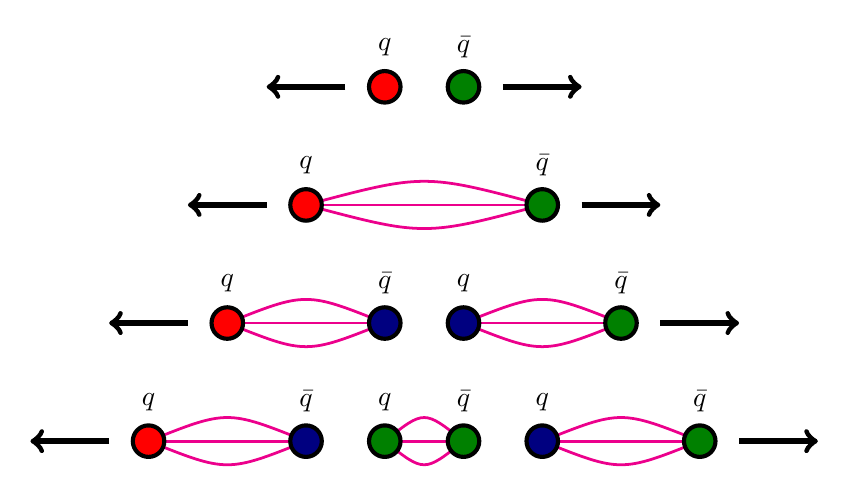
\begin{tikzpicture}[scale=1.0]
 \begin{scope}[shift={(0,0)}]
\draw[line width=2pt,black,->] (0,0)  -- +(-1,0);
\draw[fill=red,line width=1.5pt] (0.5,0) circle (0.2cm);
\draw[fill=green!50!black,line width=1.5pt]  (1.5,0) circle (0.2cm);
\draw[line width=2pt,black,->] (2,0)  -- +(1,0);
\node at (0.5,0.5) {$q$};
\node at (1.5,0.5) {$\bar q$};
\end{scope}
%%%%%%
 \begin{scope}[shift={(0,-1.5)}]
\draw[line width=1pt,magenta] (-0.5,0)  -- (2.5,0);
\draw[line width=1pt,magenta] (-0.5,0)  .. controls (1,0.4) .. (2.5,0);
\draw[line width=1pt,magenta] (-0.5,0)  .. controls (1,-0.4) .. (2.5,0);
\draw[line width=2pt,black,->] (-1,0)  -- +(-1,0);
\draw[fill=red,line width=1.5pt] (-0.5,0) circle (0.2cm);
\draw[fill=green!50!black,line width=1.5pt]  (2.5,0) circle (0.2cm);
\draw[line width=2pt,black,->] (3,0)  -- +(1,0);
\node at (-0.5,0.5) {$q$};
\node at (2.5,0.5) {$\bar q$};
\end{scope}
%%%%%%
 \begin{scope}[shift={(0,-3)}]
\draw[line width=1pt,magenta] (1.5,0)  -- (3.5,0);
\draw[line width=1pt,magenta] (1.5,0)  .. controls (2.5,0.4) .. (3.5,0);
\draw[line width=1pt,magenta] (1.5,0)  .. controls (2.5,-0.4) .. (3.5,0);
\draw[line width=1pt,magenta] (-1.5,0)  -- (0.5,0);
\draw[line width=1pt,magenta] (-1.5,0)  .. controls (-0.5,0.4) .. (0.5,0);
\draw[line width=1pt,magenta] (-1.5,0)  .. controls (-0.5,-0.4) .. (0.5,0);
\draw[line width=2pt,black,->] (-2,0)  -- +(-1,0);
\draw[fill=red,line width=1.5pt] (-1.5,0) circle (0.2cm);
\draw[fill=green!50!black,line width=1.5pt]  (3.5,0) circle (0.2cm);
\draw[fill=blue!50!black,line width=1.5pt]  (1.5,0) circle (0.2cm);
\draw[fill=blue!50!black,line width=1.5pt]  (0.5,0) circle (0.2cm);
\draw[line width=2pt,black,->] (4,0)  -- +(1,0);
\node at (-1.5,0.5) {$q$};
\node at (3.5,0.5) {$\bar q$};
\node at (1.5,0.5) {$q$};
\node at (0.5,0.5) {$\bar q$};
\end{scope}
%%%%%%
 \begin{scope}[shift={(0,-4.5)}]
\draw[line width=1pt,magenta] (2.5,0)  -- (4.5,0);
\draw[line width=1pt,magenta] (2.5,0)  .. controls (3.5,0.4) .. (4.5,0);
\draw[line width=1pt,magenta] (2.5,0)  .. controls (3.5,-0.4) .. (4.5,0);
\draw[line width=1pt,magenta] (-2.5,0)  -- (-0.5,0);
\draw[line width=1pt,magenta] (-2.5,0)  .. controls (-1.5,0.4) .. (-0.5,0);
\draw[line width=1pt,magenta] (-2.5,0)  .. controls (-1.5,-0.4) .. (-0.5,0);
\draw[line width=1pt,magenta] (0.5,0)  -- (1.5,0);
\draw[line width=1pt,magenta] (0.5,0)  .. controls (1,0.4) .. (1.5,0);
\draw[line width=1pt,magenta] (0.5,0)  .. controls (1,-0.4) .. (1.5,0);
\draw[line width=2pt,black,->] (-3,0)  -- +(-1,0);
\draw[fill=red,line width=1.5pt] (-2.5,0) circle (0.2cm);
\draw[fill=green!50!black,line width=1.5pt]  (4.5,0) circle (0.2cm);
\draw[fill=blue!50!black,line width=1.5pt]  (2.5,0) circle (0.2cm);
\draw[fill=blue!50!black,line width=1.5pt]  (-0.5,0) circle (0.2cm);
\draw[fill=green!50!black,line width=1.5pt]  (1.5,0) circle (0.2cm);
\draw[fill=green!50!black,line width=1.5pt]  (0.5,0) circle (0.2cm);
\draw[line width=2pt,black,->] (5,0)  -- +(1,0);
\node at (-2.5,0.5) {$q$};
\node at (4.5,0.5) {$\bar q$};
\node at (2.5,0.5) {$q$};
\node at (-0.5,0.5) {$\bar q$};
\node at (0.5,0.5) {$q$};
\node at (1.5,0.5) {$\bar q$};
\end{scope}
\end{tikzpicture}
\caption{Graphical illustration of the formation of color-singlet hadrons during the hadronization process.}
\end{figure}
%%%%%%%%%%%%%%%  END FIGURE  %%%%%%%%%%%%%%%%%%%%%%%%%%%%%%
%

\end{document}
